\section{Introduction}
\label{sec:intro}
Deep neural models have shown to be effective in 
a large variety of natural language inference~(NLI)
tasks~\cite{bowman2015large,wang2018glue,mostafazadeh2016corpus,roemmele2011choice,zellers2018swag}. Many of these tasks
are discriminative by nature, such as predicting a class label or
an outcome given a textual context.
%, as shown in the following example:
%\begin{example}\label{exp:snli}
%An example in SNLI.\\
%\textbf{Premise}: A swimmer playing in the surf watches a low flying airplane headed inland. \\
%\textbf{Hypothesis}: Someone is swimming in the sea.\\
%\textbf{Label}: a) Entail. b) Contradict.  c) Neutral.
%\end{example}
%The number of candidate labels may vary. 
Human solve such questions easily by
reasoning the logical connections between the premise and the hypothesis.

However, recent work~\cite{naik2018stress,schuster2019towards} 
has found that some NLP models can solve the question
fairly well by looking only at the hypothesis (or ``conclusion'' in some work)
in the datasets. 
It is widely speculated that this is because in many datasets, 
the hypothesis are manually crafted and may contain statistical artifacts 
that would be predictive of the correct answer. 
Models may learn these {\em biased features} instead of learning 
to really reason.  

\begin{figure}[th]
\centering
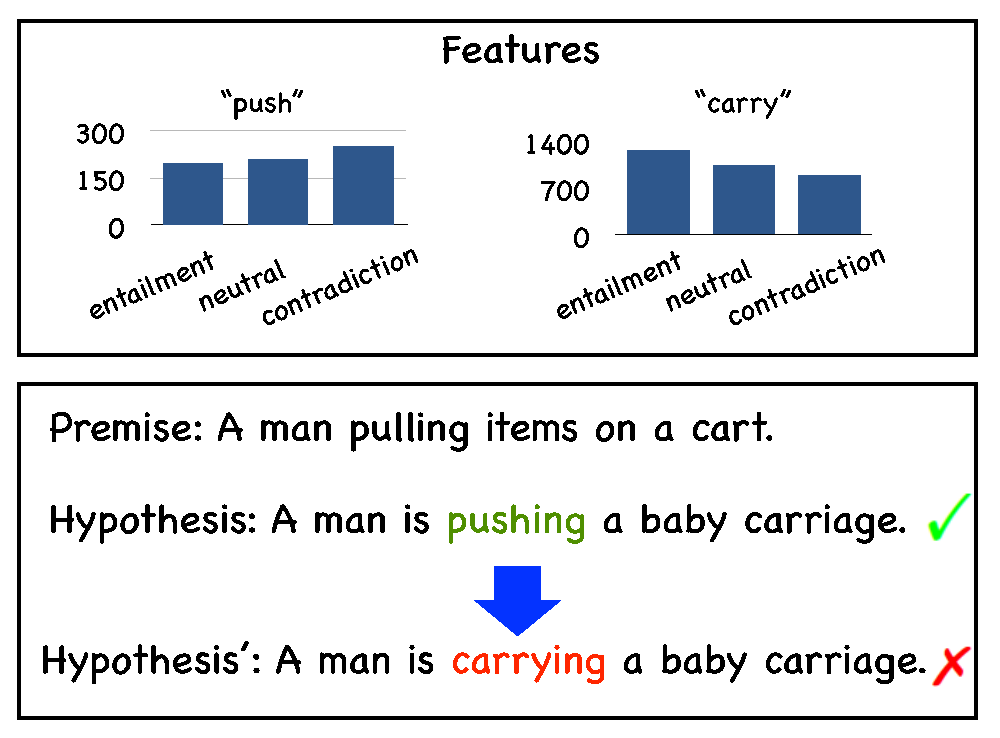
\includegraphics[width=0.8\columnwidth]{picture/example.eps}
\caption{An SNLI example. BERT can make the right prediction
(\checksymbol) on ``pushing'' but wrong (\crosssymbol ) on ``carrying''.}
%\KZ{Center ``push'' in the above. Use full words entailment, neutral, contradition. If too long, make the words slanted.}}
\label{fig:cue_def}
\end{figure}

To illustrate that such biases in the dataset are really picked up and
used by the model, we show in~\figref{fig:cue_def} the probabilistic 
distributions of the words ``push'' and ``carry'' over the 
three labels: \textit{entailment}, \textit{contradiction} and 
\textit{neutral} from SNLI~\cite{bowman2015large} training set 
and then a question from SNLI test set. The BERT model~\cite{devlin2018bert}  
makes the correct prediction \textit{contradiction} on that question. 
But once we change the word ``pushing''
to ``carrying'' without changing the meaning of the sentence, BERT
makes the wrong prediction.  
This clearly indicates that the model is affected by a single word feature. 
%In addition, the word ``pushing'' usually appears with \textit{contradiction} label. This bias information
% is probably the reason for the right choice.
%we draw the attention map between the words in
%the full question from the final encoder layer of
%the model in~\figref{fig:cue_def} for BERT~\cite{devlin2018bert} on COPA~\cite{zhou2020towards} causal reasoning task. 
%The diagram clearly shows that there’s
%virtually no connection between one choice and
%the context when the model is processing the full
%question, while the attention between the words
%within the choice remains the same when the
%model processes only the choices without the context. 
%Such ``hypothesis-only'' tests can identify problematic questions
%in the dataset if the question can be answered correctly without 
%the premise. While such a method to evaluate the quality of
%a dataset is theoretically sound, 
%it i) usually relies on training a heavy-weight model such as BERT, which
%is very costly, ii) does not provide explanation why the question is 
%a culprit.
%, and iii) cannot be used to evaluate a model since a model that
%can make a correct prediction using only the hypothesis is not necessarily a
%bad model: it is just not given the right data.  


%argumentation~\cite{niven2019probing}, commonsense reasoning~\cite{}, 
%reading comprehension~\cite{lai2017race}, question answering~\cite{talmor2019commonsenseqa} 
%and dialogue analysis~\cite{lowe2015ubuntu}. 

Inspired by black-box testing in software engineering, 
CheckList~\cite{checklist2020acl} is a framework that assesses the weakness of 
models without the need to know the details of the model. It does so by
providing additional stress test cases according to predefined 
linguistic features. Unfortunately, CheckList requires manual annotation 
of templates to generate test cases, which is not a fully automated process. 
Furthermore, it can only tell you what the model is incapable of doing but can't tell 
you what the model has learned from the data.

Here we propose ICQ (``I-See-Cue''), 
an open source profiling framework~\footnote{The address of of ICQ is 
\url{http://202.120.38.146:3308/eval/model}} that
{\em automatically} captures statistical label biases in
models for discriminative NLI tasks. %which
%In this paper, we propose a light-weight framework called
%can evaluate both the {\em data set} and the {\em model} for
%discriminative NLI tasks {\em fully} automatically. 
Recent study~\cite{gururangan2018annotation,sanchez2018behavior,poliak2018hypothesis} 
found that 
statistical bias, which are linguistic features such as 
sentiment, repetitive words and even shallow n-grams in 
benchmark datasets can be unusually correlated with specific
labels, especially the correct answers. 
In this paper, we call such label biases that are {\em actually used} by 
a model {\em cues}.  

%We call such biases artificial spurious \textit{cues} when
%they appear both in the training and test datasets with a similar distribution
%over the prediction values.
%We illustrate this in~\figref{fig:cue_def}. 
In this work, we discover cues by flattening the suspected feature distribution 
in the test data, resulting in what we call ``stress test'',
and test the model on the stress test. A cue is confirmed if 
the distribution of the same feature in the prediction results
resembles its distribution in the training data. More details
will be presented next.

%Inspired by the black-box testing in CheckList, 
%%whwith various of perturbation strategies, like typos, 
%we propose to generate test cases by just 
%filtering the original test data into new subsets according to 
%specific linquistic features, like word, NER, Negation, and sentiment, etc. 
%%in constructing the spurious cues. 
%We can show the cases distribution on each label indicates whether 
%the dataset is balance on this feature. In another word, we can 
%find the bias and cues intuitively. 
%Meanwhile,  we can prob what bias features the model really sensitive to.
%We even out the filtered test date on different labels. The even out version 
%can be used as a ``feature test'' to estimate whether a model consider 
%bias features in training data to make prediction.
%
%Our framework can be used to identify simple but effective biases and cues  
%in a broad range of multiple choice NL reasoning datasets.
%Though not all multiple choice questions in these dataset involve 
%all three components, i.e., a premise, a hypothesis and a label, 
%we will describe in~\secref{sec:formulation} how to normalize them into
%the standard form. 

%The relative size of hard part over the whole
%data indicates the quality of the dataset .
%\KZ{pls quickly finish the remaining part of intro. 
%The contributions part is critical.}
%Thus we can
%separate the original dataset into easy and hard part with 
%the bias score feature of cues
%any   dataset into easy and hard part
%and thus we can evaluate the ``biasness'' and ``quality'' of the dataset. 



%using simple and cost-effective linear classification models 
%on the simple cue features,
%which trained with unbalanced score of cues to several benchmark datasets across 
%various tasks and domains. 
%We evaluate the effectiveness of our methods with the 
%deviation between our results and random selection results. 
%Simultaneously, the test set can be divided into two parts: \textbf{easy} and \textbf{hard}. 
 %\textbf{balance} and \textbf{imbalance} are relative rather than absolute. 
%\KZ{Improving the neural models by splitting the training set.} 

%The training data can be separated into $n$ parts, test on one part and training 
%the model on the rest for each time. 
%The filtered part contains the instances 
%which can not be correctly chosen.
%The filtered data will be used to train a better model for target tasks. 

In summary, this paper makes the following contributions:
%\KZ{These contribs need to be revised right?}
\begin{itemize}
%\item we provide a light-weight but effective method to evaluate to what extent 
%NLI datasets contain statistical biases and cues;
%(\secref{sec:result}).
\item we develop an approach to assess if a model takes advantage 
of any label biases to make predictions and find out these cues;

\item we provide a demo to visually show results on a series of 
popular NLI tasks and models. 
\end{itemize}
% (\secref{sec:result}).

%\item We filter the training data and get a better performance on the \textbf{hard} dataset.
%to get a high quality training dataset which
 %is possibly closer to the intended task. 

















